\section{Grundlagen}

\subsection{Problemstellung}

In der vorangegangenen Arbeit, \textbf{T3\_3100}, wurden bereits grundlegende Funktionen des Hochregallagers implementiert und erweitert. Dazu zählen insbesondere die Prozesse:
\begin{itemize}
	\item Einlagern
	\item Auslagern
	\item Umlagern
\end{itemize}

Die Ein- und Auslagerprozesse wurden dabei vollständig umgesetzt, während die Funktion \textbf{Umlagern} im Rahmen der genannten Arbeit neu eingeführt wurde.\\\\
Im Fokus der vorliegenden Arbeit steht nun die Erweiterung des bestehenden Auslagerprozesses hin zu einer \textbf{auftragsbasierten Auslagerung}. Ziel ist es, eine realitätsnahe Abbildung industrieller Logistikprozesse zu ermöglichen, bei der Auslagerungen nicht mehr manuell, sondern basierend auf konkreten Aufträgen erfolgen.\\\\
Zur Umsetzung dieses Ansatzes wird ein \textbf{Scanner} eingesetzt, welcher das Einlesen von Bauteil- oder Artikelcodes ermöglicht. Diese Codes dienen als Grundlage für die Zuordnung und Identifikation von Lagergütern innerhalb des Systems.\\\\
Ergänzend dazu wird eine \textbf{externe Datenbankanbindung} realisiert, welche eine Synchronisation zwischen den erfassten Scandaten und den zugehörigen Auftragsinformationen erlaubt. Dadurch kann eine automatisierte und auftragsbezogene Auslagerstrategie umgesetzt werden.

Ein wesentlicher Bestandteil dieser Erweiterung ist der Einsatz der Programmiersprache \textbf{Python}. Im Gegensatz zur reinen SPS-Programmierung ermöglicht Python die Verarbeitung komplexerer Datenstrukturen sowie eine flexible Anbindung externer Systeme, wie beispielsweise Datenbanken oder Visualisierungstools.

Durch die Auslagerung von komplexeren Logik- und Datenverarbeitungsprozessen in eine Hochsprache kann die Programmstruktur auf der SPS bewusst vereinfacht gehalten werden. Dies führt zu einer besseren Überschaubarkeit, Wartbarkeit und Erweiterbarkeit des Gesamtsystems.\\\\
Im folgenden Abschnitt wird der Stand der Technik betrachtet. Dabei werden die wesentlichen Grundlagen und Technologien vorgestellt, die für die Umsetzung der auftragsbasierten Auslagerung erforderlich sind. Die grundlegenden Lagerprozesse selbst werden an dieser Stelle nicht erneut behandelt, da diese bereits in der Dokumentation zur \textbf{T3\_3100} ausführlich beschrieben sind.
\input{T3200_Kapitel Grundlagen/Lagerprozesse}
\subsection{Auftragsbasierte Prozesse}
\subsubsection{Grundprinzip der auftragsbasierten Lagerung}
Die auftragsbasierte Lagerung ermöglicht es dem Benutzer, den Lagerprozess nicht mehr durch direkte Eingaben, sondern über definierte Aufträge zu steuern.\\
Im Falle der manuellen Lagerung gibt der Benutzer seinen gewünschten Lagerplatz vor. Alternativ besteht die Möglichkeit, ein bestimmtes Bauteil auszuwählen, woraufhin der entsprechende Prozess initiiert wird.\\
Bei der auftragsbasierten Lagerung wird der Lagerprozess hingegen über ein \textbf{Eingabegerät} gesteuert. Dabei erfolgt die Eingabe nicht mehr positionsorientiert, sondern auftragsorientiert.\\

Ein Auftrag enthält die notwendigen Informationen zur Identifikation eines Lagergutes, beispielsweise eine Artikel- oder Bauteilnummer. Auf Grundlage dieser Informationen übernimmt das System die weitere Verarbeitung und trifft eigenständig Entscheidungen hinsichtlich der Lagerbewegung.\\
In vielen Fällen werden diese Informationen über eine Datenbank bereitgestellt, wodurch eine flexible und modulare Anpassung der Auftragsstruktur jederzeit möglich ist.\\

Die logische Verarbeitung der Aufträge erfolgt dabei softwareseitig, während die physische Umsetzung weiterhin durch die speicherprogrammierbare Steuerung (SPS) realisiert wird. Dadurch entsteht eine klare Trennung zwischen Entscheidungslogik und Anlagensteuerung.\\

Der Ablauf eines solchen Prozesses beginnt mit der Erfassung eines Auftrags, beispielsweise durch das Einlesen eines Codes mittels Scanner. Anschließend wird dieser Auftrag verarbeitet und die entsprechenden Lageroperationen werden automatisch ausgelöst.\\

Ziel dieser Vorgehensweise ist es, manuelle Eingriffe zu reduzieren, die Prozesseffizienz zu steigern sowie eine höhere Nachvollziehbarkeit und Fehlerreduktion innerhalb der Lagerlogistik zu gewährleisten.
\subsubsection{Ablauf der auftragsbasierten Lagerung}

Der Ablauf der auftragsbasierten Lagerung basiert auf dem Zusammenspiel mehrerer Systemkomponenten, welche unterschiedlichen Ebenen zugeordnet sind\cite{Grundlagen_Logistik}. Diese Ebenen umfassen sowohl die Eingabe- und Verarbeitungsebene als auch die Steuerungs- und Ausführungsebene der Anlage. Ziel dieser Struktur ist es, die einzelnen Prozessschritte klar voneinander zu trennen und die Datenflüsse innerhalb des Systems transparent darzustellen.\\

Im Gegensatz zu klassischen Lagerprozessen erfolgt die Steuerung hierbei nicht direkt durch den Bediener, sondern durch eine softwaregestützte Verarbeitung von Auftragsdaten. Diese Daten werden zunächst erfasst, anschließend verarbeitet und schließlich an die Steuerungsebene übergeben.\\\\
In Abbildung \ref{fig:systemaufbau} ist der grundlegende Aufbau des Systems dargestellt. Der Signalfluss beginnt bei der Eingabe, beispielsweise durch einen Scanner, und verläuft über die Verarbeitungsebene, welche durch eine Programmanwendung (z.B. Python) realisiert wird. Innerhalb dieser Ebene erfolgt auch die Synchronisation mit einer Datenbank sowie die Visualisierung über ein HMI. Anschließend werden die verarbeiteten Daten an die SPS übertragen, welche den physikalischen Teil des Prozesses übernimmt.
\begin{figure}[H]
	\centering
	\begin{tikzpicture}[
		node distance=2cm,
		>=latex,
		font=\small,
		every node/.style={align=center}
		]
		
		% Nodes
		\node (scanner) [draw, rectangle, fill=blue!10, minimum width=3.5cm, minimum height=1cm] 
		{Input\\Scanner (RS232/USB)};
		
		\node (python) [draw, rectangle, fill=green!10, below=of scanner, minimum width=4cm, minimum height=1cm] 
		{Programmanwendung\\(Python)\\Datenverarbeitung};
		
		\node (db) [draw, rectangle, fill=yellow!20, right=4cm of python, minimum width=3.5cm, minimum height=1cm] 
		{Datenbank\\(Aufträge / Artikel)};
		
		\node (sps) [draw, rectangle, fill=orange!10, below=of python, minimum width=3.5cm, minimum height=1cm] 
		{SPS\\(z.\,B. Siemens S7-1500)};
		
		\node (actuator) [draw, rectangle, fill=red!10, below=of sps, minimum width=3.5cm, minimum height=1cm] 
		{Aktorik\\(Motor / Lagerbewegung)};
		
		\node (hmi_sps) [draw, rectangle, fill=gray!15, right=4cm of sps, minimum width=3cm, minimum height=1cm] 
		{HMI\\(SPS-seitig)};
		
		% Verbindungen
		\draw[->, thick] (scanner) -- (python) node[midway, right]{RS232};
		
		\draw[->, thick] (python) -- (sps) node[midway, right]{Snap7 / TCP};
		\draw[->, thick] (sps) -- (python);
		
		\draw[->, thick] (sps) -- (actuator) node[midway, right]{Digital I/O};
		
		\draw[->, thick] (sps) -- (hmi_sps) node[midway, above]{PROFINET};
		
		\draw[->, thick] (python) -- (db) node[midway, above]{Abgleich};
		\draw[->, thick] (db) -- (python);
		
	\end{tikzpicture}
	\caption{Systemaufbau der auftragsbasierten Lagersteuerung}
	\label{fig:systemaufbau}
\end{figure}

Wie in Abbildung \ref{fig:systemaufbau} ersichtlich, erfolgt der Ablauf weitgehend seriell. Das bedeutet, dass die einzelnen Prozessschritte nacheinander durchlaufen werden und die Daten schrittweise von der Eingabe bis zur SPS weitergegeben werden. Die SPS stellt dabei die zentrale Schnittstelle zwischen der softwarebasierten Verarbeitungsebene und der physikalischen Anlagenebene dar.\\

Im ersten Schritt erfolgt die Eingabe eines Bauteilcodes, beispielsweise durch das Scannen eines Barcodes. Diese Eingabe wird von der Programmanwendung erfasst und weiterverarbeitet.\\

In der Verarbeitungsebene werden die eingelesenen Daten bereinigt und interpretiert. Auf Basis des Codes erfolgt ein Abgleich mit den in der Datenbank hinterlegten Informationen. Dadurch kann bestimmt werden, welches Bauteil ausgelagert werden soll und welche Lagerposition zugeordnet ist.\\

Nach erfolgreicher Verarbeitung werden die benötigten Steuerinformationen über eine geeignete Kommunikationsschnittstelle an die SPS übertragen. Hierbei kommen je nach System beispielsweise Protokolle wie Snap7 oder ADS zum Einsatz.\\

Die SPS übernimmt anschließend die Ansteuerung der Aktorik. Diese führt die physikalische Bewegung innerhalb des Lagersystems aus, beispielsweise das Verfahren eines Motors oder das Bewegen eines Zylinders zur Auslagerung des gewünschten Bauteils.\\

Die folgenden Abschnitte orientieren sich am in Abbildung\ref{fig:systemaufbau} dargestellten Systemaufbau und beschreiben die einzelnen Komponenten sowie deren Funktion innerhalb des Gesamtsystems.

\subsection{Identifikationssysteme (Scanner)}
\subsubsection{Allgemeine Einordnung}
Die eindeutige Identifikation von Bauteilen ist ein grundlegender Bestandteil logistischer Prozesse. Diese Identifikation kiann über unterschiedlichste Verfahren erfolgen. Die gängigste Prüfung erfolgt durch \textbf{Scanner}.\\
Automatisierte Systeme benötigen eine klare Zuordnung von Objekten um richtig arbeiten zu können. In der Logistik ist dies von besonders hoher Bedeutung.\\
Ohne eine solche Identifikation ist keine auftragsbasierte Steuerung möglich und es kann zu erheblichen Komplikationen kommen.
\subsubsection{Scanner als Identifikationssystem}

Die Aufgabe eines Einlesegerätes besteht darin, Daten schnell und zuverlässig zu erfassen. Zum Einlesen beziehungsweise zur Eingabe von Daten stehen verschiedene Möglichkeiten zur Verfügung:
\begin{itemize}
	\item Eingabe über Tastatur 
	\item Einlesen über ein Scan-Gerät
	\item Erkennung des Bauteils über eine Kamera
\end{itemize}

Im Logistikbereich müssen Daten in der Regel schnell und fehlerfrei übertragen werden. Für diese Anwendung eignen sich Scanner besonders gut. Diese sind einfach in der Handhabung und ermöglichen eine schnelle Erfassung von Daten. Im Gegensatz zur Eingabe über die Tastatur ist keine manuelle Eingabe erforderlich, wodurch Fehler reduziert werden können.\\

Zur Identifikation werden Codierungen benötigt. In der Regel werden hierfür Barcodes oder QR-Codes verwendet.\\
Im Folgenden ist eine Übersicht über die wichtigsten Merkmale und Unterschiede von \textbf{QR-Codes} und \textbf{Barcodes} dargestellt:

\begin{table}[H]
	\centering
	\renewcommand{\arraystretch}{1.3}
	\begin{tabular}{|p{4cm}|p{4.5cm}|p{4.5cm}|}
		\hline
		\textbf{Merkmal} & \textbf{Barcode} & \textbf{QR-Code} \\ \hline
		Struktur & Eindimensional (1D) & Zweidimensional (2D) \\ \hline
		Datenspeicher & Geringe Datenmenge & Hohe Datenmenge \\ \hline
		Leserichtung & Nur horizontal lesbar & Aus allen Richtungen lesbar \\ \hline
		Fehlerkorrektur & Kaum vorhanden & Integrierte Fehlerkorrektur \\ \hline
		Verwendung & Artikeletiketten, Lager & Industrie, Tracking, Datenübertragung \\ \hline
		Informationsgehalt & Meist nur ID / Nummer & Kann komplexe Daten enthalten \\ \hline
	\end{tabular}
	\caption{Vergleich von Barcode- und QR-Code-Systemen; Quelle: \cite{Codes}}
	\label{tab:Codes}
\end{table}

In Tabelle \ref{tab:Codes} werden die wesentlichen Unterschiede zwischen Barcode- und QR-Code-Systemen dargestellt. Während Barcodes aufgrund ihrer einfachen Struktur hauptsächlich zur Identifikation von Artikeln verwendet werden, bieten QR-Codes aufgrund ihres zweidimensionalen Aufbaus die Möglichkeit, deutlich mehr Informationen zu speichern.\\

Für industrielle Anwendungen, wie beispielsweise in automatisierten Lagersystemen, werden in vielen Fällen weiterhin Barcodes eingesetzt, da diese für die eindeutige Identifikation von Bauteilen ausreichend sind und sich durch eine einfache Implementierung auszeichnen. In komplexeren Anwendungen können jedoch auch QR-Codes verwendet werden, insbesondere wenn \subsubsection{Funktionsweise eines Scanners}

Der Einlesevorgang bei einem Scanner erfolgt über ein optisches Verfahren, welches je nach Bauart auf Licht-, Laser- oder Kameratechnologie basiert. 
Beim Lichtverfahren wird das Objekt gleichmäßig ausgeleuchtet, während beim Laserverfahren ein gebündelter Lichtstrahl über den Code geführt wird. Kamerabasierte Systeme arbeiten hingegen mit Bildsensoren und erfassen den Code flächenhaft.\\

Allen Verfahren gemeinsam ist die Auswertung von Hell-Dunkel-Unterschieden, welche die codierten Informationen repräsentieren.\\

Der Ablauf des Einlesevorgangs lässt sich wie folgt beschreiben:
\begin{itemize}
	\item 1. Beleuchtung des Codes durch Licht- oder Laserquelle
	\item 2. Erfassung der reflektierten Lichtanteile durch einen Sensor
	\item 3. Unterscheidung zwischen hellen und dunklen Bereichen des Codes
	\item 4. Umwandlung der optischen Signale in elektrische Signale
	\item 5. Verarbeitung und Interpretation als Zahlen- oder Zeichenfolge
\end{itemize}

Die erzeugte Zeichenfolge entspricht dabei der im Code enthaltenen Information, beispielsweise einer Artikelnummer oder Bauteilkennung. Diese kann anschließend von nachgelagerten Systemen weiterverarbeitet werden.

\begin{figure}[H]
	\centering
	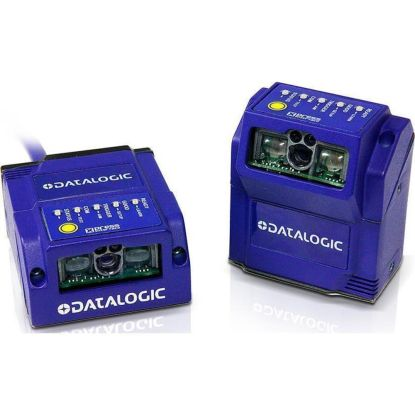
\includegraphics[width=0.3\textwidth]{images/Matrix200.jpg}
	\caption{Kamerabasierter Scanner\cite{Datalogic}}
	\label{fig:MatrixGrundlagen}
\end{figure}
\subsubsection{Datenübertragung / Schnittstelle}

Die Datenübertragung erfolgt in der Regel seriell an ein übergeordnetes System. Die erfassten Daten werden unmittelbar nach dem Einlesevorgang an die Steuerung, beispielsweise einen PC oder eine SPS, weitergeleitet. Die Ausgabe erfolgt üblicherweise als Zeichenkette (String).\\
Je nach Datenformat sind Anpassungen innerhalb der Steuerung oder durch eine zwischengeschaltete Software erforderlich, um eine korrekte Weiterverarbeitung der Daten zu gewährleisten. Am Ende des Scanwertes befindet sich in der Regel ein Abschlusszeichen, beispielsweise \texttt{"\textbackslash n"} oder ein "\texttt{Enter"}-Signal.\\

Die \textbf{Schnittstelle} kann je nach Scannerart unterschiedlich ausgeführt sein. Häufig werden RS232 sowie USB verwendet. Während RS232 eine klassische serielle Schnittstelle darstellt, kann USB durch die Emulation eines virtuellen COM-Ports ebenfalls wie eine serielle Schnittstelle verwendet werden.\\

Im Folgenden sind die wichtigsten Eigenschaften und Unterschiede beider Anschlussarten dargestellt:

\begin{table}[H]
	\centering
	\renewcommand{\arraystretch}{1.3}
	\begin{tabular}{|p{4cm}|p{4.5cm}|p{4.5cm}|}
		\hline
		\textbf{Merkmal} & \textbf{RS232} & \textbf{USB} \\ \hline
		Übertragungsart & Klassisch seriell & Paketbasiert (virtuell seriell möglich) \\ \hline
		Schnittstelle & Physischer COM-Port & Virtueller COM-Port (häufig) \\ \hline
		Datenrate & Niedrig bis mittel & Hoch \\ \hline
		Verzögerung & Sehr gering & Gering \\ \hline
		Implementierung & Einfach, robust & Etwas komplexer \\ \hline
		Verwendung & Industrie / Automatisierung & PC-Systeme / moderne Geräte \\ \hline
	\end{tabular}
	\caption{Vergleich der Schnittstellen RS232\cite{rs232_mikrocontroller} und USB\cite{usb_standard}}
	\label{tab:schnittstellen}
\end{table}

Aus Tabelle \ref{tab:schnittstellen} wird deutlich, dass beide Schnittstellen ihre Berechtigung im industriellen Umfeld besitzen. Während RS232 besonders durch seine einfache und robuste Struktur überzeugt\cite{rs232_mikrocontroller}, bietet USB eine höhere Datenübertragungsrate und wird häufig durch virtuelle COM-Ports in bestehende Systeme integriert\cite{usb_standard}.\\

Schlussendlich werden die erfassten Daten über eine Programmanwendung, beispielsweise in Python oder C, weiterverarbeitet. Dabei können projektabhängige Anpassungen vorgenommen werden, um die Daten entsprechend aufzubereiten. Die eigentliche Prozesslogik wird somit softwareseitig realisiert, wodurch automatisierte Abläufe, wie beispielsweise die Zuordnung von Bauteilen anhand von Scanwerten, angestoßen werden können.\clearpage
\subsubsection{Vorteile beim Einsatz eines Scanners}

Der Einsatz von Scannern bietet insbesondere im industriellen und logistischen Umfeld zahlreiche Vorteile. Im Folgenden sind die wichtigsten Aspekte übersichtlich dargestellt:

\begin{table}[H]
	\centering
	\renewcommand{\arraystretch}{1.3}
	\begin{tabular}{|p{5cm}|p{7cm}|}
		\hline
		\textbf{Vorteil} & \textbf{Beschreibung} \\ \hline
		Schnelle Datenerfassung & Scanvorgänge erfolgen in sehr kurzer Zeit und ermöglichen hohe Prozessgeschwindigkeiten \\ \hline
		Reduzierte Fehlerquote & Keine manuelle Eingabe notwendig, dadurch geringere Eingabefehler \\ \hline
		Einfache Integration & Scanner lassen sich leicht in bestehende Systeme einbinden \\ \hline
		Hohe Zuverlässigkeit & Robuste Technik, geeignet für industrielle Anwendungen \\ \hline
		Automatisierungspotenzial & Ermöglicht die direkte Weiterverarbeitung von Daten in automatisierten Prozessen \\ \hline
		Eindeutige Identifikation & Barcodes und QR-Codes ermöglichen klare Zuordnung von Bauteilen \\ \hline
		Flexibilität & Einsetzbar in verschiedenen Anwendungen und Branchen \\ \hline
	\end{tabular}
	\caption{Vorteile des Einsatzes von Scannern in automatisierten Systemen\cite{Datalogic}}
	\label{tab:vorteile_scanner}
\end{table}

Wie in Tabelle \ref{tab:vorteile_scanner} dargestellt, tragen Scanner maßgeblich zur Effizienzsteigerung in automatisierten Prozessen bei. Insbesondere die schnelle und fehlerarme Datenerfassung stellt einen entscheidenden Vorteil dar. Im Zusammenspiel mit softwarebasierten Verarbeitungssystemen können somit vollständig automatisierte Abläufe realisiert werden.
\input{T3200_Kapitel Grundlagen/Python}
\subsection{Speicherprogrammierbare Steuerungen (SPS)}

Speicherprogrammierbare Steuerungen (SPS) werden in der Industrie zur Automatisierung von Prozessen eingesetzt und bilden die zentrale Steuereinheit vieler Anlagen.\\
Sie dienen als Ersatz für aufwendig zu implementierende Relais- oder Schützschaltungen. Durch ihren Einsatz können schnellere und effizientere Abläufe innerhalb eines Prozesses realisiert werden.\\

In der modernen Industrie sind kurze Zykluszeiten erforderlich, welche mit rein hardwarebasierten Schaltungen nur schwer erreicht werden können. Eine SPS arbeitet nach einem zyklischen Prinzip, wodurch sowohl einfache als auch komplexe Prozesse in kurzen Zeitabständen ausgeführt werden können.\\

Die zyklische Abarbeitung eines Programms bedeutet, dass ein Programmablauf von Beginn bis Ende sequenziell durchlaufen und anschließend wiederholt wird. Dieser Vorgang wird als \texttt{Zyklus} bezeichnet. Die benötigte Zykluszeit ist dabei stark von der jeweiligen Anwendung abhängig. In logistischen Prozessen beeinflusst sie beispielsweise die Effizienz von Ein- und Auslagerungen, während in der Fertigung oftmals deutlich kürzere Zykluszeiten erforderlich sind\cite{Seitz.2021}.

\subsubsection{Aufgaben}

Eine klassische SPS arbeitet nach dem \textbf{EVA-Prinzip} (Eingabe – Verarbeitung – Ausgabe)\cite{EVA-Prinzip}.\\

Zu Beginn werden Eingänge wie Sensoren, Schalter oder Trigger, beispielsweise von einem Scanner, eingelesen. Diese Eingangssignale werden anschließend innerhalb eines Programms verarbeitet. Im letzten Schritt erfolgt die gezielte Ansteuerung der Ausgänge, beispielsweise zur Steuerung von Aktoren.

\subsubsection{Aufbau}

Der Aufbau einer SPS ist in der Regel kompakt und modular gestaltet. Im Wesentlichen besteht eine SPS aus folgenden Komponenten\cite{Weyrich.2023}:
\begin{itemize}
	\item CPU
	\item Ein- und Ausgangsmodule
	\item Kommunikationsschnittstellen
\end{itemize}

Die zentrale Verarbeitung erfolgt innerhalb der CPU. Diese verarbeitet die Eingangssignale und steuert auf Basis des Programms die Ausgänge an. Kommunikationsschnittstellen ermöglichen die Verbindung zu externen Systemen, beispielsweise zu einem \textbf{Human Machine Interface (HMI)} oder einem externen Rechner.

\subsubsection{Eigenschaften}

Speicherprogrammierbare Steuerungen weisen eine Reihe spezifischer Eigenschaften auf. Sie sind besonders robust und für den industriellen Einsatz ausgelegt. Eine wesentliche Eigenschaft ist die \textbf{Echtzeitfähigkeit}, welche die Einhaltung definierter Zykluszeiten sicherstellt\Cite{Seitz.2021}.\\

Zusätzlich verfügen viele moderne SPS-Systeme über redundante Komponenten. Dies bedeutet, dass wichtige Systemteile mehrfach vorhanden sind, um die Funktionsfähigkeit der Anlage auch im Fehlerfall aufrechtzuerhalten\cite{Seitz.2021}.

\subsubsection{Bezug zur auftragsbasierten Steuerung}

Im Rahmen der auftragsbasierten Steuerung übernimmt die SPS die Ausführung des physikalischen Prozesses. Die übergeordneten Steuerinformationen werden dabei von einer externen Programmanwendung bereitgestellt.\\

Ziel ist es, die SPS-Programmierung möglichst einfach zu halten. Komplexe Datenverarbeitungsaufgaben, wie beispielsweise die Verarbeitung von Datenbankinhalten oder die Kommunikation mit externen Systemen, werden dabei auf einen externen Rechner ausgelagert.\\

In der industriellen Praxis werden jedoch häufig Kompromisse eingegangen. Teilweise werden auch komplexere Datenstrukturen direkt innerhalb der SPS verarbeitet. Dies kann jedoch die Wartbarkeit und Fehlersuche erschweren und sollte daher nur in begrenztem Umfang erfolgen.\\

Moderne SPS-Systeme bieten die Möglichkeit, mit externen Systemen zu kommunizieren. So können beispielsweise Programme in \textbf{Python} verwendet werden, um Daten aus der SPS auszulesen oder Variablen gezielt zu setzen. Dadurch entsteht eine flexible Systemarchitektur, bei der Software- und Steuerungsebene effektiv miteinander kombiniert werden\Cite{Langmann.2021}.
\subsection{Kommunikation zwischen Python und SPS}

\subsubsection{Allgemeine Einordnung}

Zur Kommunikation zwischen einer Programmanwendung und einer speicherprogrammierbaren Steuerung werden spezielle Kommunikationsprotokolle eingesetzt, welche den Datenaustausch zwischen beiden Systemen ermöglichen.\\

Moderne Automatisierungssysteme sind hierbei in mehrere Ebenen unterteilt:
\begin{itemize}
	\item Steuerungsebene (SPS)
	\item IT-/Softwareebene (PC, Python)
\end{itemize}

Innerhalb der Steuerungsebene wird der Hauptprozess mithilfe von verknüpften Ein- und Ausgangssignalen gesteuert. Die IT- bzw. Softwareebene ermöglicht hingegen einen gezielten Austausch und die Verarbeitung von Informationen, beispielsweise die Verwaltung von Lagerdaten oder Aufträgen.\\

Der Datenaustausch umfasst dabei verschiedene Informationsarten:
\begin{itemize}
	\item Steuerbefehle 
	\item Statusinformationen
	\item Prozessdaten
\end{itemize}

Durch die Übergabe dieser Informationen kann ein dynamisches und automatisiertes Handling von Prozessen realisiert werden.

\subsubsection{Ziel der Kommunikation}

Die Übertragung von Daten von einer Programmanwendung, beispielsweise in \textbf{Python}, an die SPS ermöglicht eine weitergehende Automatisierung von Prozessen. Dabei entfällt die manuelle Eingabe von Werten, wodurch Fehler reduziert und Abläufe beschleunigt werden können.\\

Die SPS übernimmt weiterhin die kontinuierliche Steuerung der Anlage, während komplexere Datenverarbeitungsprozesse extern abgewickelt werden. Zusätzlich besteht die Möglichkeit, Status- und Fehlermeldungen aus der SPS auszulesen und weiterzuverarbeiten.\\

Ein beispielhafter Ablauf gestaltet sich wie folgt:

\begin{center}
	\texttt{Scan $\rightarrow$ Python $\rightarrow$ SPS $\rightarrow$ Auslagerung}
\end{center}

\subsubsection{Kommunikationsarten}

Für den erfolgreichen Austausch von Informationen ist eine geeignete Kommunikationsart erforderlich. Grundsätzlich lassen sich zwei wesentliche Arten unterscheiden:

\begin{itemize}
	\item Serielle Kommunikation (z.B. RS232)
	\item Netzwerkbasierte Kommunikation (z.B. TCP/IP)
\end{itemize}

Serielle Schnittstellen werden häufig für die direkte Anbindung von Geräten wie Scannern verwendet. Für die Kommunikation zwischen einer Programmanwendung und der SPS wird in der Regel eine netzwerkbasierte Kommunikation über Ethernet eingesetzt. Diese ermöglicht einen schnellen und flexiblen Datenaustausch zwischen mehreren Systemteilnehmern.

\subsubsection{Kommunikationsprotokoll Snap7}

Für den Datenaustausch zwischen einer Siemens-SPS und externen Anwendungen stehen verschiedene Kommunikationsmöglichkeiten zur Verfügung. Eine verbreitete Lösung ist die Open-Source-Bibliothek \textbf{Snap7}.\\

Snap7 basiert auf dem S7-Kommunikationsprotokoll und ermöglicht es, von externen Anwendungen – beispielsweise in Python – direkt auf Speicherbereiche der SPS zuzugreifen.\\

Zu den wichtigsten Funktionen von Snap7 zählen:
\begin{itemize}
	\item Lesen von Daten aus der SPS
	\item Schreiben von Daten in die SPS
	\item Zugriff auf Merker, Ein- und Ausgänge sowie Datenbausteine
\end{itemize}

Durch die Nutzung von Snap7 kann eine Programmanwendung gezielt Variablen innerhalb der SPS setzen oder auslesen. Dies ermöglicht beispielsweise das Starten eines Prozesses auf Basis eines eingelesenen Scanwertes.\\

Im Vergleich dazu verwendet der Hersteller Beckhoff das Kommunikationsprotokoll \textbf{ADS}, welches eine ähnliche Funktionalität bietet und ebenfalls den Zugriff auf Steuerungsvariablen erlaubt.\\

Die Verwendung solcher Protokolle ermöglicht eine klare Trennung zwischen Steuerungslogik und Datenverarbeitung. Während die SPS für die zeitkritische Anlagensteuerung verantwortlich ist, übernimmt die externe Software komplexe Datenverarbeitungsaufgaben.\\

Durch diese Struktur entsteht eine flexible und erweiterbare Systemarchitektur, welche besonders für auftragsbasierte Prozesse in der Logistik geeignet ist.\\

Die im vorliegenden Abschnitt beschriebenen Grundlagen bilden die Basis für die in den folgenden Kapitel dargestellte Konzeptentwicklung- und Umsetzung des Systems. Dabei wird insbesondere auf die konkrete Integration der einzelnen Komponenten eingegangen.